

%!TEX root = ./main.tex
\chapter{Introduction\label{Introduction}}
\section{Motivation}

% Problem: Connectivity problems exist
The end-to-end connectivity of hosts is the key service of the Internet.
However, even after 40 years of intense engineering efforts, this connectivity
is temporally broken for various reasons, such as link or hardware failure
\citep{Markopoulou:2008}, mis-configurations \citep{Mahajan:2002}, or natural
disasters \citep{Dainotti:2012:EBH,Schulman:2011}. 

% (Centrality Claim) Why do we care: Requires Troubleshooting Tools (TST) to minimize costs
This shows that there is a real need for methods to systematically detect and
locate Internet outages of remote autonomous systems, subnets, and even single
hosts. This is particularly true for Internet service providers (ISP), as for
example costumers are generating costs for time intensive debugging and support
by complaining at the ISP for unreachable networks or the ISP is contractually
liable for unreachable networks. An automated, ongoing detection and tracking of
connectivity issues of the Internet may generate transparent outage information
for customers and enables the ISP to react adequately on a detected reachability
problems if possible, for example by changing routes in case of a failure of a
transit provider. 

% (What is missing) Introduce the gap that we plan to close: 
Researches and industrial vendors have proposed various approaches for
systematically detect, locate and troubleshoot Internet outages and loss of
end-to-end reachability.

% State clearly what is missing
However, most of these approaches rely on control-plane information as BGP
routing messages or data-plane information achieved by active probing. Both
approaches not perfectly suitable for practical usage.

% bash: control plane approaches & active probing approaches
As shown by \citet{Bush:Optometry}, packets in the Internet do not necessarily
follow the control plane due to default routes. Moreover, connectivity issues
imposed by packet filtering cannot be tracked by control plane approaches
\citep{Dainotti:2011:ACI}. Besides legal issues, active probing requires the
cumbersome of target selection and increased the load on Internet
infrastructure. Furthermore, there is still no active approach which scales well
enough for the entire IPv6 address space. Moreover, both approaches are unable
to track which part of the Internet is currently actively used by their internal
clients. This is required to determine the amount of affected internal clients
and therefore to assess the urgency of the outage event. For example, as long as
a connectivity issue occurs within an unused remote network, the operator can
handle this event with low priority and fix more urgent problems first.

To fill this gap, Schatzmann et al. proposed the fully passive approach called
FACT \citep{SchatzmannPAM2011} relying on flow level information to identify
remote connectivity problems. The basic idea of FACT is to match the
corresponding outgoing and incoming flow to a bidirectional connection. Then the
remaining unidirectional connections or unresponsive connections are extracted
and investigated. The detection of an outage is consolidated by aggregating
these unresponsive connections to host, network and AS level and rating the
severity of the events by affected users. This consolidation is required to
reduce the noise of unresponsive connections caused by scanning or botnets and
implies an implicit prioritization of events which affect many internal network
users.

\citet{SchatzmanThesis2012} proposed to treat certain types of Internet
services differently because they do not require constant reachability. For
example, Skype or BitTorrent applications that are often executed on client
machines such as Desktops, Laptops, or Smartphones are likely to be reachable
only for a limited time during a day.
This characteristic is caused by the fact that these machines are often
disconnected from the network to save power or due to mobility effects. However, 
this temporal unreachability is not noticed as a problem by end-users. 
Therefore, issues of such client machine based services should not be treated 
the same way as server machine based services.

Currently, FACT does not differentiate the kind of service for tracking 
connectivity issues. This leads to the problem that client based services which 
are designed to be temporarily unavailable are wrongly interpreted as network 
outage. At the moment, FACT is dealing with this problem by three different 
approaches. 
Firstly, FACT monitors in a first step only traffic towards stable services. At  
the moment, this is heuristically defined by the traffic going to a remote TCP 
port 80 traffic from an internal client high port, representing the assumption 
that this kind of traffic is destined for a legitimate and stable web server 
socket. This approach can be viewed as preselecting only the traffic destined 
for stable services.  
Secondly, a network is only declared as unreachable if and only if all 
connection endpoints located in this network are not responding resembling a 
kind of network based traffic aggregation. 
In addition, a detected network outage is rated by the number of internal users 
which are affected by this specific outage and thus prioritizing relevant 
network outages.

\begin{figure}
	[ht] \centering
	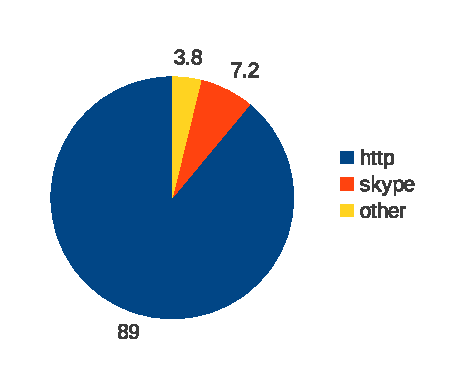
\includegraphics[width=6cm]{images/application_fact_port_80.eps}
	\caption{Application traffic running on TCP port 80 \citep{SchatzmanThesis2012}} 
	\label{fig:tcp_port80}
\end{figure}

However, by performing deep packet inspection \citet{SchatzmanThesis2012} has 
shown that the heuristic port based traffic preselection is not ideal, since a 
handful other applications are running on TCP port 80, mainly for firewall 
avoidance purposes. 
As shown in figure \ref{fig:tcp_port80}, the most 
relevant application besides HTTP which is running on TCP port 80 is Skype with 
a share of $7.2\%$ of all TCP port 80 traffic. 

This port 80 based Skype traffic yields a completely different reachability 
characteristic. As shown by figure \ref{fig:skype_traffic}, there is a 
significantly higher amount of Skype TCP port 80 sockets not reachable than 
"normal" web server sockets of content distribution networks (\emph{CDN}). This exacerbates the reliable detection of network outages. 


\begin{figure}
	[ht] \centering
	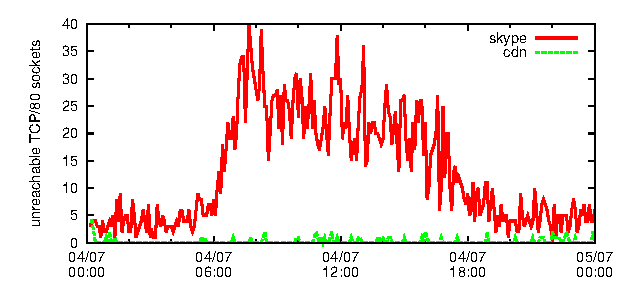
\includegraphics[width=12cm]{images/application_fact.eps}
	\caption{Unreachable TCP port 80 sockets differentiated by Skype and CDN application running on these sockets. \citep{SchatzmanThesis2012}} 
	\label{fig:skype_traffic}
\end{figure}

To this end, this thesis proposes a new type of traffic preselection which 
includes only traffic towards stable and reliable services. This is achieved by 
selecting traffic based on the past stability and popularity characteristics of 
remote services instead of the current heuristic port-based traffic preselection.

In detail, remote services are monitored and analyzed on longer time scales so
that the deduced statistical information allows the characterization of the services. Consequently, only traffic towards sockets which are characterized as stable are monitored by FACT. For example, a remote web server used only by
few users that is often unreachable, e.g. due to testing or resource scarcity,
should not be monitored by FACT. In contrast, a popular content distribution host that was always reachable in the past is more relevant. 

To sum up, the overall goal of this thesis is to extend FACT with a service
monitoring and classification functionality to enhance the current rudimentary 
traffic preselection. In fact, this functionality should enable FACT to focus 
even better on relevant connectivity issues which are related to a stable and 
popular service.

%Nevertheless, FACT's outage detection is solely based on traffic to TCP port 80 in the hope that the process listening to port 80 is a stable service, e.g. a web server. Since TCP traffic to port 80 is sometimes used by various application protocols different than HTTP, e.g. Skype, to traverse firewall and NAT devices, this assumption is not true in general. Depending on the kind of service or application, the characteristics of its stability and uptime differ significantly, i.e. if a host is a web server providing important content which should be up most of the time, or in the case of a Skype node, which are sytematically changing over time. However, from a flow perspective the connections to a Skype super-node or to a web server look very similar and are often indistinguishable.
%For this reason, the services behind the traffic which FACT is using for outage detection have to be monitored on a longer time scale and are characterized by its stability, relevance and popularity. Afterwards, from these characterized services a smart selection of stable and representative targets is created and fed into FACT for tracking remote connectivity issues. To this end, the observed traffic used for the outage detection can be generalized such that not only traffic to TCP port 80 is considered anymore. 
%The Internet is interconnecting networks all over the world since more than 40 years by 2012. The end-to-end reachability of hosts has always been a basic service of the Internet. However, this reachability is sometimes disrupted for various reasons, such as link or router collapses\citep{}, natural disasters\citep{}, political revolutions\citep{} and human errors\citep{}. There is a real need for methods to systematically detect and locate Internet outages of remote autonomous systems, subnets, and even single hosts if they are of importance. This is particularly true for Internet service providers (ISP), as for example costum·ers are generating costs for time intensive debugging and support by complaining at the ISP for unreachable networks or the ISP is contractually liable for unreachable networks. An automated, ongoing detection and tracking of connectivity issues of the Internet may generate transparent outage information for customers and enables the ISP to react adequately on a detected reachability problems if possible, for example by changing routes in case of a failure of a transit provider. As outlined in section \ref{sec:related_work} in detail, researches and industrial vendors have proposed various approaches for systematically detect, locate and troubleshoot Internet outages and loss of end-to-end reachability. However, most of these approaches rely on control-plane information as BGP routing messages or data-plane information achieved by active probing. For this reason, FACT was introduced by \citet{Schatzmann:PAM} as a flow-based approach of connectivity tracking. This is a fully passive approach for identifying remote connectivity problems and relies solely on flow-level information of cross-border network traffic. This The detection of a outage is consolidated by aggregating the unresponsive hosts to network and AS level and rating the severity of the events by affected users.
%An obvious caveat of this approach lies in the misinterpretation of service failures to host failures in case no other service is running on the observed host. This problem also exists on higher aggregation level, i.e. if a single host fails the entire network / AS is wrongly detected as down. This is even worse if this service or host is very popular with regard to internal network users. Depending on the kind of service, this may be a real problem, i.e. if this host is a web server providing important content, or may be negligible because the service or application connecting to this service is already handling this service outage as in the case of a Skype super-node. However, from a flow-point of view the connections to a Skype super-node or to a web server looks very similar and are often indistinguishable. For this reason, services have to be views at a longer time scale in order to detect services which can be characterized as stable and thus relevant for outage analysis. 
\section{Related Work 
\label{sec:related_work}} 
\subsection{Reachability
Tracking}

% Connection Tracking (Active & Passive)
Severe disruptions of the Internet's end-to-end connectivity is not a new
phenomenon, there have been connectivity outages since it early beginning as
research project. Despite that the end-to-end connectivity is a very basic
service of the Internet, the Internet community has not a deeply founded
understanding of the problems that causes its disruption \citep{Bush:Optometry}.
A dominant share of researchers focussed on "pathological behavior related to
the address space, e.g. bogon advertisements \citep{Feamster:2005}, prefix
hijacking \citep{Zhang:2010}, BGP misconfigurations \citep{Mahajan:2002} or DDoS
attacks \citep{Chen:2001}"\citep{Bush:Optometry}.

Basically, reachability can be viewed from two perspectives: data-plane and
control-plane measurements. The former mentioned studies are mainly based on
control-plane information as publicly available BGP data for deducing knowledge
about reachability. \citet{Bush:Optometry} pointed out that tracking data-plane
reachability with control-plane information is heavily inaccurate due to the
effect of secret peering policies, e.g. default routing which allows packets to
reach their destination even when a route failed to propagate through BGP.
\citet{Bush:Optometry} stated that even very basic data-plane measurements
produce better views on reachability than BGP observations. However,
control-plane based measurements are not limited to BGP data,
\citet{Markopoulou:2008} classified failures in a IP backbone network with IS-IS
information and tried to characterize these failures by layers as router,
optical/link and maintenance. To sum up, control-plane measurements of
reachability are indirect and thus of limited practical usage for systematical
reachability tracking.

% I-Seismograph(J. Lî)
In contrast, measurements of the data-plane are direct and can be more accurate
regarding end-to-end connectivity. Data-plane measurements can be divided into
active probes and passive monitoring. Whereas active probes generates additional
traffic towards the observed address space of the Internet, passive monitoring
relies fully on the traffic generated by servers and clients of the network.

Active probing is widely used for end-to-end reachability problem detection,
ranging from rudimentary debugging tools as ping \citep{PING}, paris traceroute
\citep{traceroute} or nmap \citep{Nmap} to highly sophisticated, automated
outage detection tools as Hubble \citep{Katz:2008}, PlanetSeer
\citep{Zhang:2004}. \citet{Bush:Optometry} pointed out there exist some
important limitations as filtered packets by firewall and NAT devices or
suboptimal routing which result in intermittent problems as packet rerouting.
Furthermore, there is no active probing technique known which is able to record
the return path in addition to the forward-path which can be extracted for
example with traceroute probes. It is not generally true to deduce that
forward-path reachability implies return-path reachability as well, since there
may be intermittent problems caused by suboptimal routing
\citep{Bush:Optometry}.

% Pingin' in the rain (Schulman/Spring)
\citet{Quan12a} implemented an Internet outage detection engine which is able to
actively probe an representative part of the Internet and correlate outage
events with control-plane information. This is achieved by an sophisticated
target selection approach. However, this approach is avoiding some of the
drawbacks of active probing as blockage by firewalls and NAT devices by clearly
state that they are able to track the "analyzable" IPv4 address space of the
Internet which represents the space which is really scannable by active probes.
The future scalability of this approach -- especially with respect to IPv6 -- is
questionable. 

%_--- PASSIVE --
Besides the big amount of different approaches using active probing, only few
approaches are using passive monitoring for reachability tracking.
\citet{Dainotti:2011:ACI} presented an approach for an in-depth analysis of
connectivity outages caused by political censorship by combining observations
from BGP data and data-plane information as backscatter measurements of the UCSD
network telescope and active probing data from Ark. Remarkable is their approach
of (passively) monitoring of the unsolicited data plane traffic that shed light
on Libya's attempts on deploying packet filters for enforcing the Internet
censorship. They concluded that this unsolicited and unwanted traffic captured
by network telescopes may "illuminate many different types of macroscopic
events, including but not limited to broad-scale packet-filtering-based
censorship, which is not observable by BGP data."\citep{Dainotti:2011:ACI}.

% evtl iatmon noch..
%\citet{SchatzmannPAM2011} aim to detect reachability problem by passively monitoring data-plane measurement and aggregate unresponsive connection attempts on network- and AS-level.
\subsection{Service Detection} 

% Service Detection (Active & Passive, completeness vs. scalability / importance)
The discovery and characterization of services in the Internet is most
successfully done on a massive scale, ironically not by researchers but by worms
and other malware\citep{Chen:2007}. Generally, service detection methods can be
divided into two approaches: passive monitoring and active probing. 

As \citet{Bartlett07b} pointed out that active probing is able to detect all
visible and scannable services, which is thus invasive and legally constrained.
On the other hand, passive monitoring is able to find transient services, but
fails to detect idle services. In their work, they compared the "accuracy of
passive and active approaches to service discovery and showed that they are
comlimentary"\citep{Bartlett07b}. They concluded that for best results multiple
active scans are combined with a long lasting passive monitoring. 

\citet{Leonard:2010} developed an Internet-wide service scanner called
IRLscanner. They designed their scanner to maximize politeness at remote
networks by smartly choose scanning rates. 

% Webster active / passive
\section{Contribution 
\label{sec:contribution}}
\vbox{
This master thesis contributions are the following: 
\begin{itemize}
	\item qualitative analysis of remote server sockets found by a passive approach based on \citet{Schatzmann:Mining,Schatzmann:Dissection, Schatzmann:Tracing} regarding their characteristics of stability, visibility and popularity.
	\item synthesis of the findings of this characterization for enhancing the traffic selection for tracking remote connectivity issues based on the approach of \citet{SchatzmannPAM2011} 
\end{itemize}}

\section{Outline
\label{sec:outline}}
\todo{line me out..} 
